\chapter{Apéndice A. Diagrama de clases.}

Este apendice está dedicado a los diagramas de clases de la implementación de la visualización computacional.
${ }$\\

El diagrama de clases está dividido en varias imagenes para que pueda ser visto con claridad. Ya que, debido a su tamaño las letras no serían distinguibles.
${ }$\\

\begin{figure}[h]
	\begin{center}
		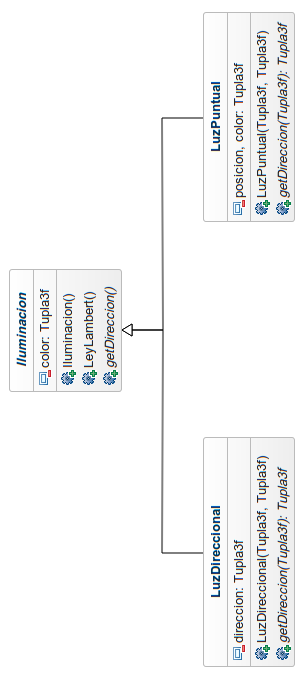
\includegraphics[width=0.6\textwidth]{imagenes/diagrama-clases-iluminacion.png}
	\end{center}
	\caption{Diagrama de clases. Herencia clase abstracta "Iluminacion".}
	\label{fig:etiq_31}
\end{figure}

\begin{figure}[h]
	\begin{center}
		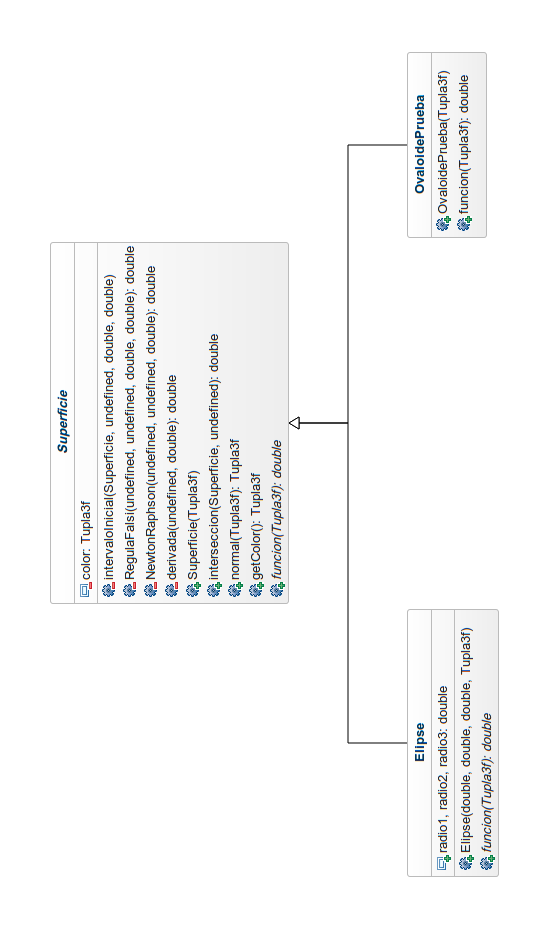
\includegraphics[width=1.0\textwidth]{imagenes/diagrama-clases-superficie.png}
	\end{center}
	\caption{Diagrama de clases. Herencia clase abstracta "Superficie".}
	\label{fig:etiq_32}
\end{figure}

\begin{figure}[h]
	\begin{center}
		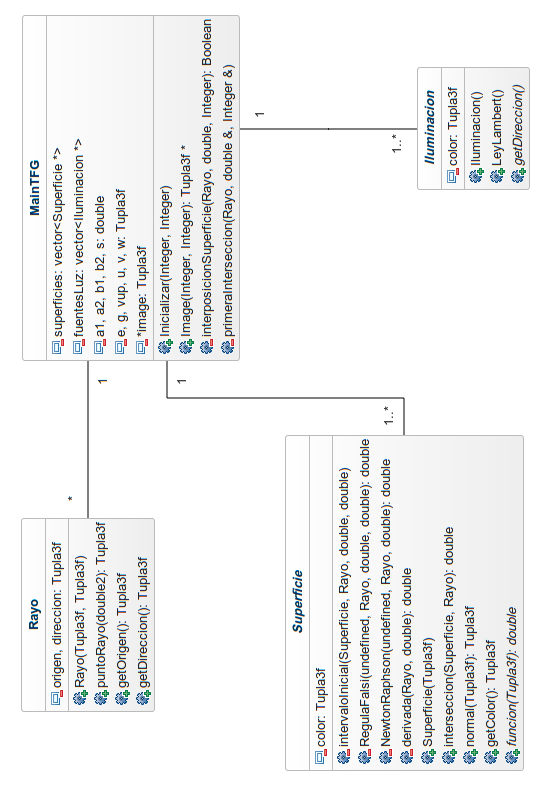
\includegraphics[width=1.0\textwidth]{imagenes/diagrama-clases-completo.png}
	\end{center}
	\caption{Diagrama de clases.}
	\label{fig:etiq_33}
\end{figure}